The following test was performed to verify the correctness of the pixel
association process. 
The differenc of intensity at corresponding pixels in the original images
$I_{j}$ and rectified images $I_{j}^{rect}$ are given by:

\begin{align}
  \Delta I_{1,i} &= I_1(u_{1,i}) - I_1^{rect}(w_{1,i}) \\
  \Delta I_{2,i} &= I_2(u_{2,i}) - I_2^{rect}(w_{2,i}) 
  \hspace{2em} \text{for } i = 1 \ldots n 
  \hspace{1em}\text{,}
  \label{eqn:rect/I_def}
\end{align}

where $u_{1,i}$, $u_{2,i}$ denote the pixels in the original image and
$w_{1,i}$, $w_{2,i}$ denote the pixels in the rectified image. 

If the rectified pixels are computed in accordance with the rectification
process of the images given by image\_proc of ROS, we would expect both 
differences to be approximately zero, since:

\begin{align}
  I_1(u_{1,i}) &= I_1^{rect}(w_{1,i}) + \epsilon_{1,i} \\
  I_2(u_{2,i}) &= I_2^{rect}(w_{2,i}) + \epsilon_{2,i} 
  \hspace{2em} \text{for } i = 1 \ldots n
  \hspace{1em}\text{,}
  \label{eqn:rect/diffI_eq}
\end{align}

with $\epsilon_{i,j}$ the error arising solely from interpolation of the rectified
images.

The pixels of the rectified image need to obey

\begin{equation}
  w_{i,j} = P_j \begin{pmatrix} X_{i,j}^{rect} \\ 1 \end{pmatrix}
  \hspace{2em} \text{for } j = 1, 2
  \hspace{1em}\text{,}
  \label{eqn:rect/w_def}
\end{equation}

where $X_{i,j}^{rect}$ are computed such that $w_{i,j} = \tilde{u}_{i,j}$, with

\begin{align}
  \tilde{u}_{i,j} &= K'(T_j(X_i)) \hspace{2em} \text{, where} \\
  T_j(X_i) &= \pi(C_{C_j M} (X_i - {_M}r_{MC_j})) \hspace{2em} \text{and} \\
  \pi(\begin{pmatrix} x, y, z \end{pmatrix}^T) &= 
  \begin{pmatrix} x/z, y/z, z \end{pmatrix}^T 
  \hspace{1em}\text{.}
  \label{eqn:rect/utilde_def}
\end{align}

Remember that $u_{i,j}$ are given by 
\begin{equation}
  u_{i,j} = K_j (D_j(T(X_i))) 
  \hspace{2em} \text{for } i = 1 \ldots n \text{, } \hspace{1em} j = 1,2
  \hspace{1em}\text{,}
  \label{eqn/rect/u_def}
\end{equation}

which concludes the above considerations.

All tools for computing the pixel correspondences being defined, a look at 
Figures \ref{fig:rect_r1} and \ref{fig:rect_r2} shows that the resulting error
between the rectified image and the original image is indeed unformly 
small and with no patterns observable in both left and right images.
The above equations for pixel correspondences are thereby validated for the 
rectification process given by image\_proc of ROS.

\begin{figure}[h]
  \centering
  \begin{subfigure}[b]{0.49\textwidth}
    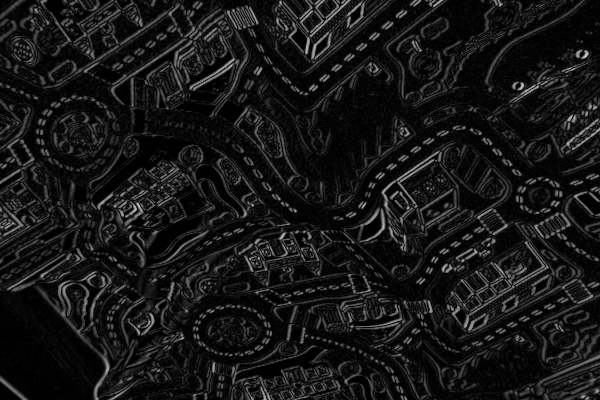
\includegraphics[width=\textwidth]{figures/rect_r1.jpg} 
    \caption{Left image (mean: 22.67)} 
    \label{fig:rect_r1}
  \end{subfigure}
  \begin{subfigure}[b]{0.49\textwidth}
    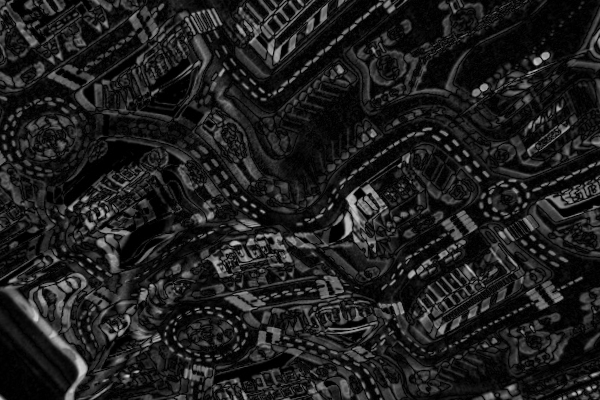
\includegraphics[width=\textwidth]{figures/rect_r2.jpg} 
    \caption{Right image (mean: 30.2813)}
    \label{fig:rect_r2}
  \end{subfigure}
  \caption{Rectification intensity errors with $n_x = 600$ and $n_y = 400$.}
\end{figure}

Similar considerations can be applied for validating the interpretation of the
camera parameters given in the camera\_info message.

The following assumptions are to be tested.

\begin{align}
  C_{SC_j} &= R_j \hspace{2em} \text{for j=1, 2} 
  \implies C_{C_2C_1} = R_2^TR_1 \hspace{2em} \text{and} \\
  _{C_1}r_{C_1C_2} &= \begin{pmatrix} -P_j(0,3)/P_j(0,0) & 0 & 0
  \end{pmatrix}^T
  \hspace{1em}\text{.}
\end{align}

The methodology applied is the following. If the above assumptions hold, then one 
can obtain the pixel coordinates in the second rectified image given the
coordinates in the first image using $X_{i,1}^{rect}$ such that $w_{i,1} = \tilde{u}_{i,1}$, with
$\tilde{u}_{i,1}$ defined as above, and 

\begin{align}
  X_{i,2}^{rect} &= C_{C_2C_1} (_{C_1}r_{C_1X_i} + _{C_1}r_{C_1C_2}) \\
                 &= C_{C_2C_1} (X_{i,1}^{rect} + _{C_1}r_{C_1C_2}) 
  \hspace{1em}\text{.}
  \label{eqn:rect/assumptions}
\end{align}

The residuals of the original images $I_1$ and $I_2$ and of
the rectified images $I_1^{rect}$ and $I_2^{rect}$ are given by

\begin{align}
  \Delta r_i &= I_1(u_{1,i}) - I_2(w_{2,i}) \\
  \Delta r_i^{rect} &= I_1^{rect}(w_{1,i}) - I_2^{rect}(w_{2,i})
  \hspace{2em} \text{for } i = 1 \ldots n 
  \hspace{1em}\text{.}
  \label{eqn:rect/res_def}
\end{align}

If the rectified pixels are computed in accordance with the rectification
process of the images, we have 

\begin{equation}
  \Delta r_i = \Delta r_i^{rect} + \epsilon_i  
  \hspace{2em} \text{for } i = 1 \ldots n
  \hspace{1em}\text{,}
  \label{eqn:rect/res_eq}
\end{equation}

with $\epsilon_i$ the error arising solely from interpolation errors between the
left and the right image.
The photometric error in the original and rectified image are is shown in Figures
\ref{fig:rect_ru} and \ref{fig:rect_rw}. Since at this stage, no reliable depth
theinformation is available, low photmetric errors cannot be expected, which explains 
the relatively high average value. However, from Equation \ref{eqn:rect/res_eq}
we know that the photometric errors should be approximately the same in both
cases. A visualization of the difference between the two in Figure \ref{fig:rect_rdiff} 
shows that this is indeed the case. Therefore, trnsform between the left and
right image can be computed from the camera\_info message as given in
\ref{eqn:rect/assumptions}.

\begin{figure}[h]
  \centering
  \begin{subfigure}[b]{0.49\textwidth}
    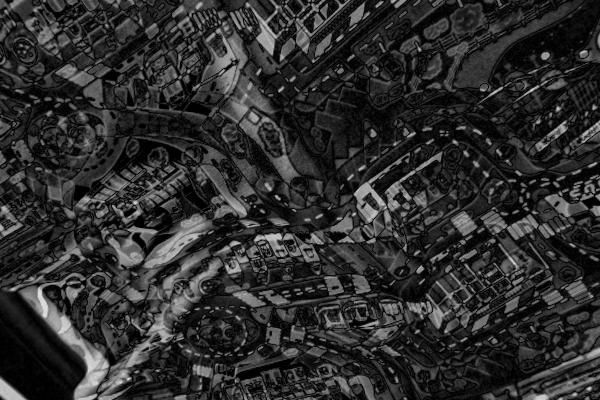
\includegraphics[width=\textwidth]{figures/rect_ru.jpg} 
    \caption{Original image (mean: 45.87)}
    \label{fig:rect_ru}
  \end{subfigure}
  \begin{subfigure}[b]{0.49\textwidth}
    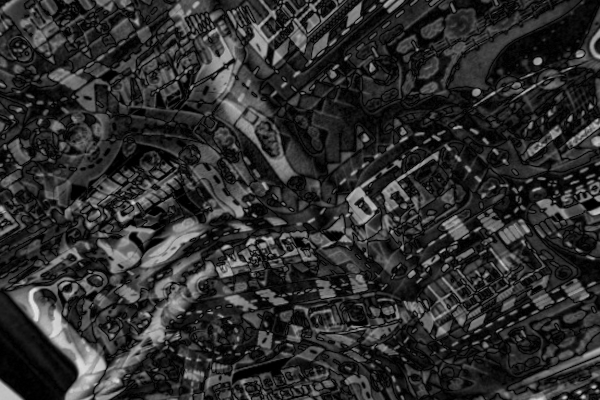
\includegraphics[width=\textwidth]{figures/rect_rw.jpg} 
    \caption{Rectified image (mean: 45.42)}
    \label{fig:rect_rw}
  \end{subfigure}
  \\
  \begin{subfigure}[b]{0.7\textwidth}
    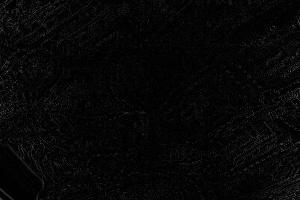
\includegraphics[width=\textwidth]{figures/rect_rdiff.jpg} 
    \caption{Difference (mean: 31.6758)}
    \label{fig:rect_rdiff}
  \end{subfigure}
  \caption{Rectification residual errors with $n_x = 600$ and $n_y = 400$.}
  \label{fig:rect}
\end{figure}

